\documentclass[letterpaper, 12pt, oneside]{report}               
% define the basic details of our document 

\newif\iffinalize
\newif\iffrontmatter
\newif\ifendmatter
\newif\ifprintversion

\finalizetrue       % lets us work on the report piecemeal style
% \frontmattertrue    % turn on/off the frontmatter
% \endmattertrue      % specific options for the paper version
% \printversiontrue   % specific options for the paper version

% \usepackage{./local_packages/macros_and_settings_simplified}
\usepackage{./local_packages/macros_and_settings_current}
% \usepackage[noreferences]{./local_packages/macros_and_settings_simplified}  % you can do this to stop it from compiling references

\addbibresource{ref.bib}
\input{./short_list.tex} % all our acronyms
\input{commands.tex}
\usepackage{listings}  
\input{template_settings.tex}
\input{define_json_listings_style}
\input{define_python_listings_style}
\lstset{style=mysimpleCodestyle}  % set default style


%\glsdisablehyper%\glsenablehyper
%\renewenvironment{Solution}[1]{\par\bigskip\nho_approx_pes.pdfoindent\phantomsection {\bfser\textbf{}ies Solution  of exercise #1}\quad}{}

% \usepackage{palatino} % the Palatino font is somewhat nice... but can cause problems at times (optional)
\newif\iffinalize
\newif\ifprintversion

\finalizetrue       % lets us work on the report piecemeal style 
% (if commented out it stops the title page and all frontmatter and other stuff from being generated, this speeds up compilation)

% \printversiontrue   % specific options for the paper version (you don't need to use until you submit for printing)

\iffinalize 
  \ifprintversion \geometry{letterpaper, left=1in, right=1in, top=1in, bottom=1in, footskip=0.25in} 
  \else           \geometry{letterpaper, left=1in, right=1in, top=1in, bottom=1in, footskip=0.25in} 
  \fi
  %\makeglossaries 
\else \fi

\begin{document}

\iffinalize \pagestyle{empty} \pagenumbering{alph}
\begin{titlepage}
        \begin{center}
        \vspace*{1.0cm}

        \Huge
        {\bf Vibronic Model Diabatization Protocols and Vibrational Electronic Coupled Cluster (VECC) Approaches Towards Spectroscopy }

        \vspace*{1.0cm}

        \normalsize
        by \\

        \vspace*{1.0cm}

        \Large
        Benny Chen \\

        \vspace*{3.0cm}

        \normalsize
        A thesis \\
        presented to the University of Waterloo \\ 
        in fulfillment of the \\
        thesis requirement for the degree of \\
        Master of Science \\
        in \\
        Chemistry \\

        \vspace*{2.0cm}

        Waterloo, Ontario, Canada, 2024 \\

        \vspace*{1.0cm}

        \copyright\ Benny Chen 2024 \\
        \end{center}
\end{titlepage}
\else \fi

% frontmatter formatting
\iffinalize\doublespacing\pagestyle{plain} \pagenumbering{roman}\setcounter{page}{2}\else \fi

\iffinalize
%\addcontentsline{toc}{chapter}{Author's Declaration} 
\vspace*{\fill}
\begin{center}\begin{minipage}{9cm}
  I hereby declare that I am the sole author of this thesis. This is a true copy of the thesis, including any required final revisions, as accepted by my examiners.  \\\\ 
  I understand that my thesis may be made electronically available to the public.
\end{minipage}\end{center}
\vspace*{\fill}
\else \fi

\iffinalize
%\addcontentsline{toc}{chapter}{Statement of Contributions}
\chapter*{Statement of Contributions} 
\else \fi

\iffinalize 
%\addcontentsline{toc}{chapter}{Abstract}
\chapter*{Abstract}%
A diabatization method utilizing GAMESS multi-configurational quasidegenerate perturbation theory for purposes of obtaining spin-orbit coupling and n-th order couplings was implemented in Python. Iron pentacarbonyl was studied with a triple zeta polarized Sapporo basis set.

\newpage%
\else \fi

\iffinalize 
%\addcontentsline{toc}{chapter}{Acknowledgements}
\chapter*{Acknowledgements} 
Neil's tips for thesis writing:
- Start out with where you are confident in, say the script and completed models
- If you get stuck on compiling say a table, just take a photo of a handwritten one and stick it in as temporary placeholder
- Have many rough passes
\newpage%
\else \fi

\iffinalize
%\addcontentsline{toc}{chapter}{Dedication}
\chapter*{Dedication} 
\else \fi

\begin{spacing}{1.15} % so the toc fits on 1 page
  \iffinalize 
  \setcounter{tocdepth}{2}%\addtocontents{toc}{\protect\setcounter{tocdepth}{0}
  \tableofcontents \newpage
  \else \tableofcontents \clearpage
  \fi
\end{spacing}
% we use mhchem package, so \ce{3H2O}

\iffinalize \addcontentsline{toc}{chapter}{List of Figures}
\listoffigures
% Human-in-the-loop vibronic model
% This means iexp should always be 1 (else MCTDH complains), and tau ~= tf
% \includegraphics[]{images/manual_supervision.png}
% \includegraphics[]{images/qsize0.3_18d_fitting_1st_mode7.png}
% \includegraphics[]{images/rhodium_xps.JPG} % https://www.hic.ch.ntu.edu.tw/PES/file/%E5%8F%83%E8%80%83%E8%B3%87%E6%96%99/XPS%20handbook.pdf
\newpage

\else \fi

\iffinalize \addcontentsline{toc}{chapter}{List of Tables} \listoftables \newpage
\else \fi

\iffinalize \addcontentsline{toc}{chapter}{List of Illustrations} \chapter*{List of Illustrations}  \newpage
\else \fi

\iffinalize \addcontentsline{toc}{chapter}{List of Abbreviations} \printglossaries  \newpage
\else \fi

\iffinalize \addcontentsline{toc}{chapter}{List of Symbols} \chapter*{List of Symbols} \textbf{SOC - Spin Orbit Coupling \\ GAMESS, GMS - General Atomic and Molecular Electronic Structure System \\ CC - ComputeCanada \\ CAS(m,n), 2e1o - Complete Active Space m Electrons and n Orbitals Configuration \\ DMO - Diabatic Molecular Orbitals \\ \\ GMC-QDPT - Generalized Multiconfiguration - Quasi-Degenerate Perturbation Theory \\ MR - Multireference \\ MC - Multiconfiguration \\ SCF - Self-consistent Field \\ FeCO - Iron Pentacarbonyl} 
https://uwaterloo.ca/chemistry/current-graduate-students/chemistry-msc-thesis-defence-timeline

\newpage
\else \fi

\iffinalize \addcontentsline{toc}{chapter}{Nomenclature} \chapter*{Nomenclature} \newpage
\else \fi

%\iffinalize \addcontentsline{toc}{chapter}{Graphic or quote} \chapter*{Graphic or quote} \newpage
%\else \fi

\newpage

\pagenumbering{arabic} % change to arabic page numbering
\setcounter{page}{1}
% all acronyms should be written out in full the first time used
% seperately in the abstract and in the main text

% Acronym definitions
%\newacronym{utc}{UTC}{Coordinated Universal Time}
%\newacronym{adt}{ADT}{Atlantic Daylight Time}
%\newacronym{est}{EST}{Eastern Standard Time}
%\gls{bbb}\gls{aaa}\gls{utc}\gls{adt}\gls{est}\gls{bbb}
% rememeber to run "makeglossaries raymond_neil" from terminal in the project folder

% --------------------------------------------------------------------------------------------------
% --------------------------------------------------------------------------------------------------
\iffinalize \chapter{Introduction} 
% --------------------------------------------------------------------------------------------------
\doublespace

% --------------------------------------------------------------------------------------------------
\section{Motivation}
% --------------------------------------------------------------------------------------------------


Goal: introduce Vibronic (vib+elec) and diabatic models / diabatization protocols -> then give some specific example of why they're cool
(why do we care (in general), and specific thing )
\begin{enumerate}
    \item BOA works for most systems, ignore specific math term
    \item BUT, for interesting systems (Nonadaibatic) it is not sufficient and so we need new approaches
    \item diabatic is one such approach, and it has various advantages.
\end{enumerate}


    \subsection{Open-shell transition metal complex spectra and thermochemistry}
    
\begin{enumerate}
    \item provide background for the general version/style (Open-shell transition metal complex) of Fe(CO)5 
    (you could mention / use the D3h systems you trained on as general examples... you don't have to, just if its useful to draw on that experience)
    
    \item introduce the specifics of Fe(CO)5 

    1,2,3,4,5,6,7,8
    somewhere in intro you should explain what CASSCF is.
    go look at CHEM gaussian course notes from jake + textbook or two (marcel/fred?/toby might have a textbook to recommmend)
    
    
    \item talk about challenges and other stuff?
    
\end{enumerate}

    Fe(CO)5
    Graham Worth (GAMESS) guy and Haruyuki Nakano (GMC-QDPT) guy did FeCO+ in 1999. Marcel wanted a large iron complex with carbonyl ligand. Carbonyls stabilize metals. Toby trained me on D3h systems. So, combining all these, we did Fe(CO)5, which is a D3h transition metal complex.


% \section{Explanation of common terms} 
% maybe need to explain CASSCF GMCPT etc..? or you could explain in the section where you introduce them
% write later if needed


% --------------------------------------------------------------------------------------------------
\section{Systems of Interest / Objectives (Most difficult system) } % maybe find different wording? 
% --------------------------------------------------------------------------------------------------


% --------------------------------------------------------------------------------------------------
    \subsection{Vibronic Models: Quadratic-order CASSCF GMCPT SOC Protocol} % Best case scenario

    Fancy method, otherwise why not just DFT B3LYP 6-31G* @ everything ...


    Analogy: we did not build the car, we merely are a driver, make sure we diligently perform routine maintenance on it, know what engine is and how to fill gas, etc. 

    We do not construct a car from the ground up, not feasible... monumental task
\newpage
\else \fi

% --------------------------------------------------------------------------------------------------
\section{Overiew of Thesis}
% --------------------------------------------------------------------------------------------------

basically you just briefly introduce each chapter and its purpose
see coco's and any body else's thesis'




% --------------------------------------------------------------------------------------------------
% --------------------------------------------------------------------------------------------------
\iffinalize \chapter{Methods and Context}
% --------------------------------------------------------------------------------------------------


% --------------------------------------------------------------------------------------------------
\section{Electronic structure theory}
% --------------------------------------------------------------------------------------------------
    \newpage
    
% --------------------------------------------------------------------------------------------------
    \subsection{TDSE, BOA}

%%%%% TAKEN FROM 494, JUST FOR REFERENCE
    Let the full molecular Schrödinger's Equation be defined as: 
\begin{equation}\label{eq:schrodinger}
    \begin{split}
        \hat{H}(\Vec{R}) \Psi_{n}(\Vec{r};\Vec{R}) = E_n \Psi_{n}(\Vec{r};\Vec{R})
    \end{split}
\end{equation}
%
The full molecular Hamiltonian:
\begin{equation}%\label{eq:eqnlabel}
    \begin{split}
        \hat{H} = -\sum_{\alpha}^{M} \frac{1}{2M_{\alpha}} \nabla_{\alpha} \cdot \nabla_{\alpha}
         -\sum_{i}^{N} \frac{1}{2m_{e}} \nabla_{i} \cdot \nabla_{i}
         + \sum_{i,j>i}^{N} \frac{1}{r_{ij}} + \sum_{i, \alpha}^{N,M} \frac{-Z_{A}}{r_{i\alpha}}
         + \sum_{\alpha, \beta \neq \alpha}^{M} \frac{Z_{A}Z_{B}}{R_{\alpha \beta}}
    \end{split}
\end{equation}
%
Which can concisely be represented by kinetic and potential energy operators $\hat{T}$ and $\hat{V}$:
\begin{equation}%\label{eq:eqnlabel}
    \begin{split}
        \hat{H} = \hat{T}_{N} + \hat{T}_{e} + \hat{V}_{ee} + \hat{V}_{Ne} + \hat{V}_{NN}
    \end{split}
\end{equation}
%
Note the subscripts $e, N$ are for electronic and nuclear correspondingly.
\begin{equation}%\label{eq:eqnlabel}
    \begin{split}
        \hat{H}_{} = \hat{T}_{N} + \hat{H}_{elec} 
    \end{split}
\end{equation}
%
\begin{equation}%\label{eq:eqnlabel}
    \begin{split}
        \hat{H}_{elec} = \hat{T}_{e} + \hat{V}_{ee} + \hat{V}_{Ne} + \hat{V}_{NN}
    \end{split}
\end{equation}
%$\hat{H}_{elec}$ critically does not include the nuclear-kinetic term $\hat{T}_{N}$. 
\\ Let the wavefunction, $\Psi$, be the sum over the electronic eigenstates $\phi_{\lambda} (\Vec{r};\Vec{R})$ and nuclear eigenstates $\chi_{\lambda} (\Vec{R})$:
\begin{equation}%\label{eq:eqnlabel}
    \begin{split}
        \Psi (\Vec{r};\Vec{R}) = \sum_{\lambda} \phi_{\lambda} (\Vec{r};\Vec{R}) \chi_{\lambda} (\Vec{R})
    \end{split}
\end{equation}
Here, $\Vec{r}$ indicates electron coordinates, and $\Vec{R}$ refers to nuclear configuration. The subscripts $\lambda$ and $\mu$ denote electronic states. To describe a parametric dependence of $\Vec{r}$ on $\Vec{R}$, $(\Vec{r};\Vec{R})$ is used. Signifying that although an explicit dependence on $\Vec{R}$ is not present in the function, $\Vec{r}$ values are predicated at a single $\Vec{R}$ parameter \cite{szabo2012modern}. Therefore, if $\Vec{R}$ changes, so does $\phi_{\lambda}(\Vec{r};\Vec{R})$. \\
Proceed with full expansion of Hamiltonian acting on the wavefunction:
\begin{subequations}\begin{align}%\label{eq:eqnlabel}
    &\hat{H} (\Vec{R}) \Psi (\Vec{r};\Vec{R})\nonumber
\\  
    &=
    \left[ 
        - \sum_{\alpha} \frac{1}{2M_{\alpha}} \Vec{\nabla_{\alpha}} \cdot \Vec{\nabla_{\alpha}}   + \hat{H}_{elec} 
    \right]
    \left[ 
        \sum_{\lambda} \phi_{\lambda} (\Vec{r};\Vec{R}) \chi_{\lambda} \Vec{(R)}
    \right]
\\
    \begin{split}
        &=
        \Big( - \sum_{\alpha} \frac{1}{2M_{\alpha}} ~\Big) \sum_{\lambda} 
        [ 
            \chi_{\lambda} \Vec{(R)} \Vec{\nabla^{2}_{\alpha}} \phi_{\lambda} (\Vec{r};\Vec{R})
            + \Vec{\nabla_{\alpha}} \phi_{\lambda} (\Vec{r};\Vec{R}) \Vec{\nabla_{\alpha}} \chi_{\lambda}
        \\  &\qquad\qquad
            + \phi_{\lambda} (\Vec{r};\Vec{R}) \Vec{\nabla^{2}_{\alpha}} \chi_{\lambda} \Vec{(R)}
            + \Vec{\nabla_{\alpha}} \chi_{\lambda} \Vec{\nabla_{\alpha}} \phi_{\lambda} (\Vec{r};\Vec{R})
            + E_{\lambda}(\Vec{R}) \phi_{\lambda}(\Vec{r};\Vec{R}) \chi_{\lambda} \Vec{(R)} 
        ]
    \end{split} 
\\  
    \begin{split}
        &=
        \Big( - \sum_{\alpha} \frac{1}{2M_{\alpha}} ~\Big) \sum_{\lambda} 
        [ 
            \chi_{\lambda} \Vec{(R)} \Vec{\nabla^{2}_{\alpha}} \phi_{\lambda} (\Vec{r};\Vec{R}) 
        \\  &\qquad\qquad
            + \phi_{\lambda} (\Vec{r};\Vec{R}) \Vec{\nabla^{2}_{\alpha}} \chi_{\lambda} \Vec{(R)} 
            + 2\Vec{\nabla_{\alpha}} \phi_{\lambda} (\Vec{r};\Vec{R}) \Vec{\nabla_{\alpha}} \chi_{\lambda} 
            + E_{\lambda}(\Vec{R}) \phi_{\lambda}(\Vec{r};\Vec{R}) \chi_{\lambda} \Vec{(R)} 
        ]
    \end{split}
\end{align}\end{subequations}
%
Integrating against $\phi_{\mu} (\Vec{r},\Vec{R})$ over all electronic coordinates, $\Vec{r}$, and asserting that these states are orthonormal at a single fixed $\Vec{R}$, produces a sum of four terms:
% a possible alternative layout to your current ABCD thing
 \begin{align} 
   \tag{\textbf{A}}\label{eq:A2}
     &= \sum_{\lambda} \int \phi_{\mu}^{*} (\Vec{r};\Vec{R}) \sum_{\alpha} - \frac{1}{2M_{\alpha}} \Vec{\nabla_{\alpha}^{2}} \phi_{\lambda} (\Vec{r};\Vec{R})~dr \chi_{\lambda} \Vec{(R)}
     %
     %
 \\  \tag{\textbf{B}}\label{eq:B2}
     %
     &\qquad+ \sum_{\lambda} \sum_{\alpha} \delta_{\lambda \mu} \frac{-1}{2M_{\alpha}} \Vec{\nabla_{\alpha}^{2}}  \chi_{\lambda} \Vec{(R)}
     %
     %
     \\  \tag{\textbf{C}}\label{eq:C2}
     %
     &\qquad+ \sum_{\lambda} \sum_{\alpha} \int \phi_{\mu}^{*} (\Vec{r};\Vec{R}) \Vec{\nabla_{\alpha}} \phi_{\lambda} (\Vec{r};\Vec{R}) dr \cdot - \frac{1}{2M_{\alpha}} \Vec{\nabla_{\alpha}} \chi_{\lambda} \Vec{(R)}
     %
     %
     \\  \tag{\textbf{D}}\label{eq:D2}
     %
     &\qquad+ \sum_{\lambda} \delta_{\lambda \mu} E_{\lambda} (\Vec{R}) \chi_{\lambda} \Vec{(R)}
     \\ &= \sum_{\lambda} E_{\lambda} \Vec{(R)}  \delta_{\lambda \mu} \chi_{\lambda} \Vec{(R)}
 \end{align}

The BOA facilitates setting the expansion in terms of a single electronic state, hence $\lambda = \mu$. Terms \textbf{A} and \textbf{C} in the BOA are also ignored. The \textbf{A} term represents a diagonal Born-Oppenheimer correction to potential, useful in specialized instances--as in accounting for different $M_{\alpha}$ (e.g. isotopes) \cite{nooijennotes}. It is typically proximate enough to zero for it to be neglected. Likewise, \textbf{C} is zero for real normalized wavefunctions. \textbf{C} is referred to as the off-diagonal non-adiabatic coupling (NAC) terms. In other words, only \textbf{B} and \textbf{D} terms remain because terms with the presence of $\int dr \Vec{\nabla_{\alpha}} \phi_{\lambda} (\Vec{r};\Vec{R})$ are effectively zero if there exists little change in $\phi_{\lambda}$ with respect to $\Vec{R}$, thus implying no coupling between electronic wavefunctions and nuclear configuration \cite{nooijennotes}. 
\\
As for a small example, so far the BOA shows:
\begin{equation}%\label{eq:eqnlabel}
    \begin{split}
        \begin{bmatrix}
            \hat{T}_N + E_{1}(\Vec{R}) + A_{1}(\Vec{R}) & N.A.C.\\
            N.A.C.& \hat{T}_N + E_{2}{(\Vec{R}) + A_{2}(\Vec{R})}
        \end{bmatrix}
    \end{split}
\end{equation}

Ultimately, the Schrödinger equation with the BOA applied appears as:
\begin{equation}\label{eq:10}
    \begin{split} 
            \left[ \hat{T}_N + E_{\lambda} \Vec{(R)} \right] \Psi_{\lambda, n} \Vec{(R)} = E_{n} \Psi_{\lambda. n} \Vec{(R)}
    \end{split}
\end{equation}
Where label $n$ is for rotational-vibrational levels and recalling $\lambda$ is for electronic states. Attention to the term $E_{\lambda}(\Vec{R})$, which is a function of nuclear configuration. %Unlike the case for the full molecular Schrödinger equation, where energy is a constant (which is not a functional of coordinates), 
$E_{\lambda}(\Vec{R})$ is defined to be a single point sufficiently able to define a potential energy surface (PES), $E_{\lambda}(\{ \Vec{R} \})$. Now the electronic wavefunction $\phi_{\lambda} (\Vec{r};\Vec{R})$, wavefunction $\chi_{n} (\Vec{R})$ (detailing nuclear motion), and potential energy surface $E_{\lambda} \Vec{(R)}$ in \Cref{eq:10} can be solved for  at a single electronic state $\lambda$ with any given fixed-geometry $\Vec{R}$. In practice of using BOA concepts, \Cref{fig:fig1} demonstrates how the electronic ground state PES can be theoretically constructed. Understanding surfaces in this fashion gives rise to adiabatic states or true Born-Oppenheimer surfaces \cite{villanueva2020spectroscopic}. 
\\


\newpage
% -------------------------------------------------------
\subsection{Adiabatic and Diabatic Basis Connection}
% -------------------------------------------------------
%Focus is now directed towards excited states. 
Earlier discussions on the importance of non-adiabatic dynamics to vibronic models and spectra can now deepen. Although the BOA was highlighted to reduce calculation complexity (i.e. avoiding evaluation of integral terms), it fails when the NACs are relevant--\Cref{fig:fig2}(a), occurring mainly in two situations:
\begin{enumerate}[label=\roman*.]
    \item The adiabatic state character changes rapidly as a function of geometry.
    \item Degenerate electronic states, separations on the order of vibrational energy level values.
\end{enumerate}

When these conditions exist, Yarkony has described how conical intersections and avoided crossings between separate single excited states develop, and in order to simulate spectra successfully, the model needs to account for neglected terms and be governed by multiple PES to describe nuclear motion \cite{yarkony2001conical}. %The BOA simply cannot be applied anymore. This indicates a departure from the adiabatic (BOA) basis, namely to a non-adiabatic process that requires invoking diabatic states. %Vibronic coupling theory can assist in simulating the non-adiabatic system.
\\ 
Recall, term \textbf{C} contains an integral, which is inversely proportional to energy separation:
\begin{equation}\label{eq:inverseproportional}
    \begin{split}
            \int \phi_{\mu}^{*} (\Vec{r};\Vec{R}) \Vec{\nabla_{\alpha}} \phi_{\lambda} (\Vec{r};\Vec{R})~dr 
            \propto \frac{1}{E_{\mu} - E_{\lambda}}
    \end{split}
\end{equation}

Ultimately, the Schrödinger equation with the BOA applied appears as:
\begin{equation}\label{eq:10}
    \begin{split} 
            \left[ \hat{T}_N + E_{\lambda} \Vec{(R)} \right] \Psi_{\lambda, n} \Vec{(R)} = E_{n} \Psi_{\lambda. n} \Vec{(R)}
    \end{split}
\end{equation}

\begin{equation}\label{eq:inverseproportional}
    \begin{split}
            \int \phi_{\mu}^{*} (\Vec{r};\Vec{R}) \Vec{\nabla_{\alpha}} \phi_{\lambda} (\Vec{r};\Vec{R})~dr 
            \propto \frac{1}{E_{\mu} - E_{\lambda}}
    \end{split}
\end{equation}

\begin{equation}\label{eq:atodmatrix}
    \begin{split}
        \begin{bmatrix}
            \hat{T}_N + E_{1}(\Vec{R}) + A_{1}(\Vec{R}) & N.A.C.\\
            N.A.C.& \hat{T}_N + E_{2}{(\Vec{R}) + A_{2}(\Vec{R})}
        \end{bmatrix}
        \Rightarrow
        \begin{bmatrix}
            \hat{T}_{N} + E_{11}(\Vec{R}) & E_{12}(\Vec{R}) \\ 
            E_{21}(\Vec{R}) & \hat{T}_{N} + E_{22}{(\Vec{R})}
        \end{bmatrix}
    \end{split}
\end{equation}
%
Obtaining this matrix of diabatic form, it can be utilized to describe potentials and a coupled set of vibrational wavefunctions $\chi_a(\Vec{R})$:
\begin{equation} 
    \begin{split}
        \begin{pmatrix}
            \hat{T}_{N} + E_{11}(\Vec{R}) & E_{12}(\Vec{R}) \\ 
            E_{21}(\Vec{R}) & \hat{T}_{N} + E_{22}{(\Vec{R})}
        \end{pmatrix}
        %
        \begin{pmatrix}
            \chi_{1}(\Vec{R}) \\ 
            \chi_{2}(\Vec{R})
        \end{pmatrix} 
        = E
        %
        \begin{pmatrix}
            \chi_{1}(\Vec{R}) \\ 
            \chi_{2}(\Vec{R})
        \end{pmatrix} 
    \end{split}
\end{equation}

\begin{equation}\label{eq:diabaticstates}
    \begin{split}
            \Psi_{a}(\Vec{r};\Vec{R}) = \sum_{\lambda} U_{\lambda a} (\Vec{R}) \phi_{\lambda} (\Vec{r};\Vec{R})
    \end{split}
\end{equation}

\begin{equation}\label{eq:overlapmatrix}
    \begin{split}
            S_{\lambda \mu}(\Vec{R}) = \int \phi_{\mu}^{*} (\Vec{r};\Vec{R}_{q_0}) \phi_{\lambda} (\Vec{r};\Vec{R}_{q_0 \pm dq_{i}})
    \end{split}
\end{equation}

\begin{equation}%\label{eq:eqnlabel}
    \begin{split}
            \sum_{\lambda} \int \phi_{\mu}^{*} (\Vec{r};\Vec{R})
            %\Vec{\nabla_{\alpha}}
            \hat{H}_{elec} \Psi_{a}(\Vec{r};\Vec{R}) \phi_{\lambda} (\Vec{r};\Vec{R}) dr
            %\cdot - \frac{1}{2M_{\alpha}} \Vec{\nabla_{\alpha}}
            \chi_{\lambda} \Vec{(R)}
            = \sum_{\lambda} E_{\mu \lambda} \chi_{\lambda} \Vec{(R)}
    \end{split}
\end{equation}

\begin{equation} \label{eq:17}
    \begin{split}
            E_{\mu \lambda} (q) = E_{\mu \lambda} (0) + \sum_{i}^{M} E_{\mu \lambda}^{i}q_i + \frac{1}{2} 
            \sum_{i>j}^{M} E_{\mu \lambda}^{ij}q_{i}q_{j} + \cdots
    \end{split}
\end{equation}

\begin{equation} \label{eq:18}
    \begin{split}
            E_{\mu \lambda}^{i} = \frac{E_{\mu \lambda} (\Vec{R}_{q_0} + dq_{i}) - E_{\mu \lambda} (\Vec{R}_{q_0} - dq_{i})}{2dq_{i}}
    \end{split}
\end{equation}




    \subsection{MCSCF, CASSCF, GMC-QDPT}
        %%% TAKEN FROM PROPOSAL %%%%
        \subsubsection{Diabatic Molecular Orbitals}
        Configurational uniformity is a concept devised by Hisao Nakamura and Donald Truhlar to manufacture diabats from adiabats. In their framework, which expands on previous work by Atchity and Rudenberg, diabatization-adapted molecular orbitals (DMOs) are obtained and then subsequent DSFs (diabatic state functiosn) are constructed. The idea is to optimize for uniformity in electronic configurations that originate from DMOs. 

        \subsubsection{GMC-QDPT}
        Haruyuki Nakano and coworkers have devised the Generalized Multiconfiguration - Quasi Degenerate Perturbation Theory (GMC-QDPT) scheme. GMC-QDPT itself is classified as a composite method that aims to recover both static and dynamical correlation. The 'generalized' label refers to zero-restrictions in variational space. This means beyond CASSCF and RASSCF, so general MCSCF wavefunctions are applicable for submission as input. The QDPT latter half indicates a subsequent multireference calculation that proceeds. In short, it is intended for multistate calculations, and optimal for heavy/relativistic calculation purposes. Interestingly, when benchmarked with CAS-QDPT, there is only a 0.1 eV and 1 kcal/mol $\Delta$. Nakano has prepared an excellent student reference guide for performing GAMESS GMCPT and GMC-QDPT calculations: {https://ccl.scc.kyushu-u.ac.jp/\~nakano/gmcpt.html}. An important consideration is that FCI is often intractable due to the computational cost growing factorially in terms of reference space determinants, so this efficient scheme is more feasible instead.

        \subsubsection{Active Space Design}
        Designing the active space is a pedantic problem.
        
        Cool paper: \url{https://arxiv.org/pdf/2111.15587#:~:text=ORMAS%20is%20a%20construction%20of,and%20minimum%20number%20of%20electrons.}


%======================================================================
% \addcontentsline{toc}{section}{Introduction}
\section{Diabatization\label{sec:s1}}
%======================================================================

    Loops in python are notoriously slow. So in collaboration with Neil Raymond, we refactored the excessive looping that distorted the modes into array operations. This drastically improved the performance. Furthermore, it also made the entire program more dynamic in a sense that it can adapt and be extended for a variety of purposes. An example here is fitting. This situation arose where distortion beyond-quadratic-order at a single mode was needed, and the recasted arrays handled this trivially as compared to looping. Another key aspect of this change was the fact that the arrays forced us to understand exactly what dimensions are required in the diabatization code's various calculation modules. We have stitched together various functionalities such as: text processing, coordinate distortion, input file generation, GAMESS job submission, and operator file generation. 

    PPT idea: use opacity overlay to highlight and gray out parts of the screen for emphasis.

    We originally opted to extract data using the slow pythonic 'read' method. However, this proved to be debilitating when operating on large output files to a point where the bottleneck could be hours when running the script. Therefore we opted to use grep instead. When it came down to the full computational study on FeCO, surprisingly even grep was deemed too slow. The average size of the FeCO output file (there are ~ 1000 outputs) is 70 megabytes or around 2 million lines of text. When we grepped the SOC data, it took around 4 hours. So finally we pivoted to using memory-mapping. This not only made the program more performant, reducing the runtime of the script processing all 28 modes of FeCO from 10300 seconds (with grep) to a mere hour.

    If diabatic energy, we need to extract along the diagonal of the states array (a,a). 
    If diabatic coupling, we need to extract along the off-diagonal of the upper triangular states array (a,b). 
    This needs to be performed for linear, quadratic, and bilinear.  

    Update on May 16/17th work:
    Neil helped make it read JSON. We want to do SOC for VECC. We found incredible difficulty in making sure the JSON reads the .op model correctly due to a load of issues.


    %--------------------------------------------------------------------------------------------------------
    \subsection{Adiabats and diabats}
    %--------------------------------------------------------------------------------------------------------
    \subsection{TD-DFT excited states model limitations}

%--------------------------------------------------------------------------------------------------------
\section{Calculation of Spectra}
%--------------------------------------------------------------------------------------------------------

    
    %--------------------------------------------------------------------------------------------------------
    \subsection{Time-correlation functions}
    
    %--------------------------------------------------------------------------------------------------------
    \subsection{MCTDH}
    
    %--------------------------------------------------------------------------------------------------------
    \subsection{VECC}
    VECC Paper: https://arxiv.org/pdf/2312.14164.pdf
    Our model comparisons have the following assumptions: although we can submit more information to MCTDH than VECC (e.g. off-diagonal coupling of state energies and excited state-to-state transition dipole moments), our comparisons are limited to whatever VECC accepts. Therefore, the difficulty arises from finding a hybrid format compatible to both dynamics-simulation-schemes that can capture the model. A technical challenge, mainly.
\section{Relativistic effects}
    \subsection{Spin Orbit Coupling (SOC)}
\section{Thermal effects}
    \subsection{TF-VECC: Thermal Field Vibrational Electronic CC}
\section{Computational Details}
    \newpage
    \subsection{GAMESS-US}
    GAMESS is an ab initio quantum chemistry package. The general pipeline of how calculations are run: HF/DFT/GVB/MCSCF $\Rightarrow$ CI/MP2/CC (these are correlation corrections) $\Rightarrow$ SOC/DK (these are relativistic effect corrections)

    Having reservations about a job is needed, oftentimes a double or even triple check is prudent.
\newpage
%--------------------------------------------------------------------------------------------------------
    
\begin{table}[h!]
    \centering
    \caption[Step 1 Information]{\label{table:one} Step 1 information.}
    \begin{tabular}{ c||c|c c }
        \toprule
        Command Line & Input & Output 
    \\  \midrule\midrule
    %
        \verb|python3 step0.py| & &
    \\  & &
    \\  Manual execution: & \verb|molecule_optfreq.com| & \verb|molecule_optfreq.log| 
    \\  \verb|python3 step1.py| &  & \verb|master_values.json|
    \\  & &
    \\  Automated execution: & &
    \\  \verb|python3 automate_scripts.py -1|  & &
    \\
        \bottomrule
        \end{tabular}
\end{table}
% --------------------------------------------------------------------------------------------------
    \subsection{nlogn, ComputeCanada (Computational Resources)}
    On nlogn, the available compute is as follows:
    cpu[005-006] intel,westmere, X5670 12 48000 io003 intel,ivybridge,E5-2 16 128000 io[001-002] intel,westmere,X5670 12 48000 \\

    On ComputeCanada Graham cluster, the available compute per node is 32 CPUs with 125GB of memory. \\

    The GAMESS memory requirements for parallelized calculations is as follows: ((mwords * p + memddi)*8) / 1024 = TOTAL NUMBER OF GB. Where p is the number of processors, mwords is the amount of memory (in Words) for each processor, memddi is the distributed memory for optimization runs, and 8/1024 to account for the conversion of words to gigabytes. Therefore, on nlogn, the max amount of compute per run would be 16 CPUs at 4 gigabytes. For reference, see https://docs.alliancecan.ca/wiki/GAMESS-US. \\

    To compile Zeng's GMC-QDPT compatible GAMESS version on ComputeCanada clusters, it is complicated. First, the \textit{gmcpt.src} module must be obtained from Zeng. The next step is to \textit{module load intel/2023.2.1} and run \textit{./config} in GMS' source directory; this will prompt a set of questions in which the answers are as follows: linux64, enter, enter, enter, ifort, 10, none. After you msut enter the ddi/ directory and run ./compddi and move the ddikick executable one directory above. Finally, you must run ./lked to link GAMESS to your path.
\newpage
\else \fi

% ------------------------------------------------------------------------------------
% ------------------------------------------------------------------------------------
\iffinalize
\chapter{Vibronic Model Development}
% ------------------------------------------------------------------------------------
\newpage


% ------------------------------------------------------------------------------------
\section{Full diabatization ('model name') example} 
% the point being that you explain step-by-step how the protocol works.
% maybe one section in chapter three should be a full example of calculating water or D3h or some such model with SOC? showing the sections of the text files that you have to strip out, and the values etc.
% ------------------------------------------------------------------------------------
An explanation of the automated process of creating a vibronic model will be presented using water (H2O) as an example.
The process is a slightly modified version of the approach used in Aranda and Santoro’s work [19].
Work is being done to make the code to preform this procedure publicly available on GitHub 2.

The process has, broadly, five phases:
% add enum here
1. Section 3.5.1 Geometry optimization
2. Section 3.5.2 Calculating geometry displacements
3. Section 3.5.3 Evaluating the electronic integral (submit all gamess calculations) diabatization func
4. Section 3.5.4 Collating numerical results (and pump out .op/.json files)
...


see SECTION 2.4 in Neil's thesis


\subsection{Step 1: Geom opt + Freq}
<explain the begin, show a Z-matrix file, 
\subsection{Step 2:}
% optional sections
\subsubsection{Special details about +1/+2/+3/+4}
\subsubsection{Special details about selecting certain modes to have +8 etc}

\subsection{Step 3:Evaluating the electronic integral}
\subsubsection{Step 3: SOC flag + details}
\subsubsection{Step 3: SOC flag + details}

\subsection{Step 4:}
\subsubsection{Details about making .json file}
\subsubsection{Details about making .op file}
% \subsubsection{Details about differences between MCTDH and VECC? maybe?}


% optional section to explain assorted edge cases 
\section{Comments on further details of protocol (and other random edge cases)} 


% ------------------------------------------------------------------------------------
\section{CASSCF}
% ------------------------------------------------------------------------------------
    To elucidate the active space without prior intuition is a challenging task. Many iterations on assessing the orbitals and adjusting the dimensions of the active space were needed. This human in the loop
    
% ------------------------------------------------------------------------------------
\section{Diabatization protocol Python code explanation}
% ------------------------------------------------------------------------------------

\textit{combined\_toolkit.py} is simply a collection of 8 utilities that are useful in preparing the diabatization template:

\centering{
    (1) OPTIMIZED RHF \\
    (2) OPTIMIZED ROHF \\
    (3) Semi-canonical MOs \\
    (4) MCSCF Natural Orbitals \\
    (5) OPTIMIZED MCSCF \\ 
    (6) DMO group \\ 
    (7) REFDET GROUP \\ 
    (8) EQUILIBRIUM GEOMETRY \\
}





% \usepackage{algorithm}
% \usepackage{algpseudocode}

% \begin{algorithm}
% \caption{An example algorithm}
% \begin{algorithmic}[1]
% \\Require $n  \\geq 0$
% \\Ensure $y  =  x^n$
% \\State $y  \\gets 1$
% \\State $X  \\gets  x$
% \\State $N  \\gets  n$
% \\While{$N  \\neq 0$}
%     \\If{$N$  is even }
%         \\State $X  \\gets  X  \\times  X$
%         \\State $N  \\gets \\frac{N}{2}$
%         \\Comment{ This is a comment }
%     \\ElsIf{$N$  is odd }
%         \\State $y  \\gets  y  \\times  X$
%         \\State $N  \\gets  N  - 1$
%     \\EndIf
% \\EndWhile
% \end{algorithmic}
% \end{algorithm}



Toby Zeng created a custom DMO using symmetrized reference geometry orbitals. 39 (a1'), 45,46 (e'') 47,48 (e') 51 (a1'*) 53,54 (e'*) became the SOC's 44, 45,46, 47,48, 49, 50,51.


% if the content of the lstlisting is super long then you can simply put them in seperate files
%\input{./lst_smatrix_elements}


\newpage


% ------------------------------------------------------------------------------------
\subsection{diabatize() and mctdh() functions}
    
% ------------------------------------------------------------------------------------
\subsection{Distorting coordinates and calculating up to quadratic coupling constants}

% ------------------------------------------------------------------------------------
\subsection{Fitting on n-th order models}
Bells and whistles

% ------------------------------------------------------------------------------------
\subsection{Generating spectra via MCTDH and VECC}
To crack this problem, rewritten program with Neil. The program is not perfect, but we can still use it to do relatively functional calculations and build models.

\newpage
\else \fi


% -----------------------------------------------------------------------------------
% ------------------------------------------------------------------------------------
\iffinalize
% \chapter*{Full Computational Study on Large System}
\chapter{Application (to real world models)?}
% ------------------------------------------------------------------------------------


% ------------------------------------------------------------------------------------
\section{Details about running calculations}
% ------------------------------------------------------------------------------------
Because we run on GRAHAM and they are stupid and dumb I can't use the <x-ds32> opptino in MCTDH which makes it 1 billion times slower.
Transfer files.


% ------------------------------------------------------------------------------------
\section{Details about producing spectra}
% ------------------------------------------------------------------------------------

% ------------------------------------------------------------------------------------
\section{any other random stuff you need to explain before the systems?}
% ------------------------------------------------------------------------------------



% ------------------------------------------------------------------------------------
\section{Preliminary systems}
% ------------------------------------------------------------------------------------
brief description of each system and results you expect and this is to prove that it has no issues in easy cases.


% ------------------------------------------------------------------------------------
\subsection{H2O}
add short description of file
show table with Hamiltonian parameters
show image of molecule? (progbably unnnecessary)
show spectra from MCTDH and VECC (maybe show constant, linear, quadratic, SOC?)
discuss the results? are they identical, good this system was just top test xyz, and it behaved as we expected.


% ------------------------------------------------------------------------------------
\subsection{CH2O}
add short description of file
show table with Hamiltonian parameters
show image of molecule? (progbably unnnecessary)
show spectra from MCTDH and VECC (maybe show constant, linear, quadratic, SOC?)
discuss the results? are they identical, good this system was just top test xyz, and it behaved as we expected.




% ------------------------------------------------------------------------------------
\subsection{NH3}
add short description of file
show table with Hamiltonian parameters
show image of molecule? (progbably unnnecessary)
show spectra from MCTDH and VECC (maybe show constant, linear, quadratic, SOC?)
discuss the results? are they identical, good this system was just top test xyz, and it behaved as we expected.


Transition metals: CoF3, RhF3

% ------------------------------------------------------------------------------------
\section{Complex systems}
% ------------------------------------------------------------------------------------
%A paragraph that talks about the three systems. 
As we explained in (section intro) transition metal complexes are of high importance because <some reason>.
We primarily focused on CoF3, RhF3 and Fe(CO)5 beacuse of <some reason>.
The two smaller systems (CoF3, RhF3) are good for benchmarking the model generation as well as fine-tuning the calculation parameters for MCTDH and VECC.
The large system (Fe(CO)5) is expected to be very difficult and has only <some citation of a paper and demonstrate how its real tough and scary>


% ------------------------------------------------------------------------------------
\subsection{CoF3}
add short description of file
show table with Hamiltonian parameters
show image of molecule? (progbably unnnecessary)
show spectra from MCTDH and VECC (maybe show constant, linear, quadratic, SOC?)
discuss the results? are they identical, good this system was just top test xyz, and it behaved as we expected.

% ------------------------------------------------------------------------------------
\subsection{RhF3}
add short description of file
show table with Hamiltonian parameters
show image of molecule? (progbably unnnecessary)
show spectra from MCTDH and VECC (maybe show constant, linear, quadratic, SOC?)
discuss the results? are they identical, good this system was just top test xyz, and it behaved as we expected.

% ------------------------------------------------------------------------------------
\subsection{Fe(CO)5}
add short description of file
show table with Hamiltonian parameters
show image of molecule? (progbably unnnecessary)
show spectra from MCTDH and VECC (maybe show constant, linear, quadratic, SOC?)
discuss the results? are they identical, good this system was just top test xyz, and it behaved as we expected.

\includegraphics[width=1\columnwidth]{images/modes7to9.png}


% ------------------------------------------------------------------------------------
\subsection{Vibronic spectra of test case pnictogen hydrides}

% ------------------------------------------------------------------------------------
\subsection{Spectra of \ce{D_{3h}} SOC transition metal complexes (\ce{CoF3} and \ce{RhF3})}

% \section{Dimanganese decacarbonyl, \ce{Mn2(CO)10}}
% https://www.sciencedirect.com/science/article/pii/S0022328X12006237

\section{Iron pentacarbonyl, \ce{Fe(CO)5}}
    Using \ce{Fe(CO)5} as an example: we first recognized that the full valence active space was 11o18e. However, doing a oneshot for even the ground state equilibrium geometry calculation did not result in anywhere near convergence. Instead, we had to slowly build up the transition metal compound's ground state geometry by filling in bunches of electrons and orbitals at a time. The initial calculation was a 4+ cation, with a multiplicity of 1. Next, a calculation of 1+ charge and multiplicity of 4, due to three unpaired electrons between a set of a" and e' of orbitals 46 through 48. This calculation resolved the orbital ranking: a" was lower than e'. Finally, a third calculation was ultimately performed on the fully electron-filled molecule and this neutral model yielded the full equilibrium geometry. CHEMICAL INTUITION NEEDED!
    
    We first started by doing an optimization of \ce{Fe(CO)5^4+}. Then, we introduced 2 electrons (multiplicity of 3), and then made it neutral. Observed that the irreducible representation orbital ranking of HOMO was $e'$ and LUMO was $a_{1}'$ After obtaining the equilibrium geometry, we proceeded to fill the active space. 4o4e, 5o8e, 6o8e, 6o10e, 8o10e, 9o12e, and the finally the full valent 11o18e. However, 11o18e did not seem to converge no matter what we tried. So we opted for 8o10e to tide us over and achieve a reasonable spectrum.

    Curse of dimensionality when doing 33 modes ... gigantic ... ML-MCTDH is needed according to Prateek: https://mattermodeling.stackexchange.com/questions/535/what-is-the-largest-system-for-which-vibrationally-resolved-electronic-spectra-h \\

    So we screened modes using effective vibronic coupling magnitude above a threshold. Linear couplings only. See JCTC singlet and triplet fission paper. Heart-wrenching that MCTDH could only compile up to 220k parameters when we needed 260k for our full model. Emailed Prateek and H.D.-Meyer. We can assert that only these 12 modes belong to the model. Incredible struggle, but nah, we'd win. Selected screen modes: [7, 8, 12, 13, 15, 18, 19, 21, 22, 23, 30, 31]. 12 out of 27. TZ: show a spreadsheet of screenshots here, displaying the ones we selected, does it make sense according to out analysis? \\

    (see email with Dieter) We have good news. Prof. Meyer advised that the MCTDH-84 version I was running was outdated and that upgrading to the newest 86 version would do the trick. Fortunately Toby had a copy of 86 too on hand. Not only has the parameter limitation seemed to be resolved, but it similarly resolves a secondary issue in 84 where parallelized runs where erroring out (but works now in 86!).

    Stitching together various functionalities, tuning

    May 29th: we have done plotting of diabatic energies today and saw that mode 15 was equatorial dissociation and mode 23 was axial dissociation. Equatorial dissociation leads to one of the COs on the horizontal plane leaving, resulting in the axial COs to bend down and resulting in Td symmetry. Whereas, axial dissociation results in one CO on principal axis leaving and resulting in C3v symmetry.

    https://stackoverflow.com/questions/19412382/gnuplot-line-types#19420678

    We are using ORMAS+GMCPT!
    https://ccl.scc.kyushu-u.ac.jp/~nakano/gmcpt.html

    Normally we use Douglas-Kroll (DK) in the $\$relfwn$ group, howeveer Sapporo basis sets like RELWFN=LUT-IOTC instead.
    
    Scale breaks things. We have to fix things, redesign, change this, change that...

    
\includegraphics[width=1\columnwidth]{images/op_FeCO3Q_17st_PBF7_tf100.00_xyz_spectrum_1900by900.png}

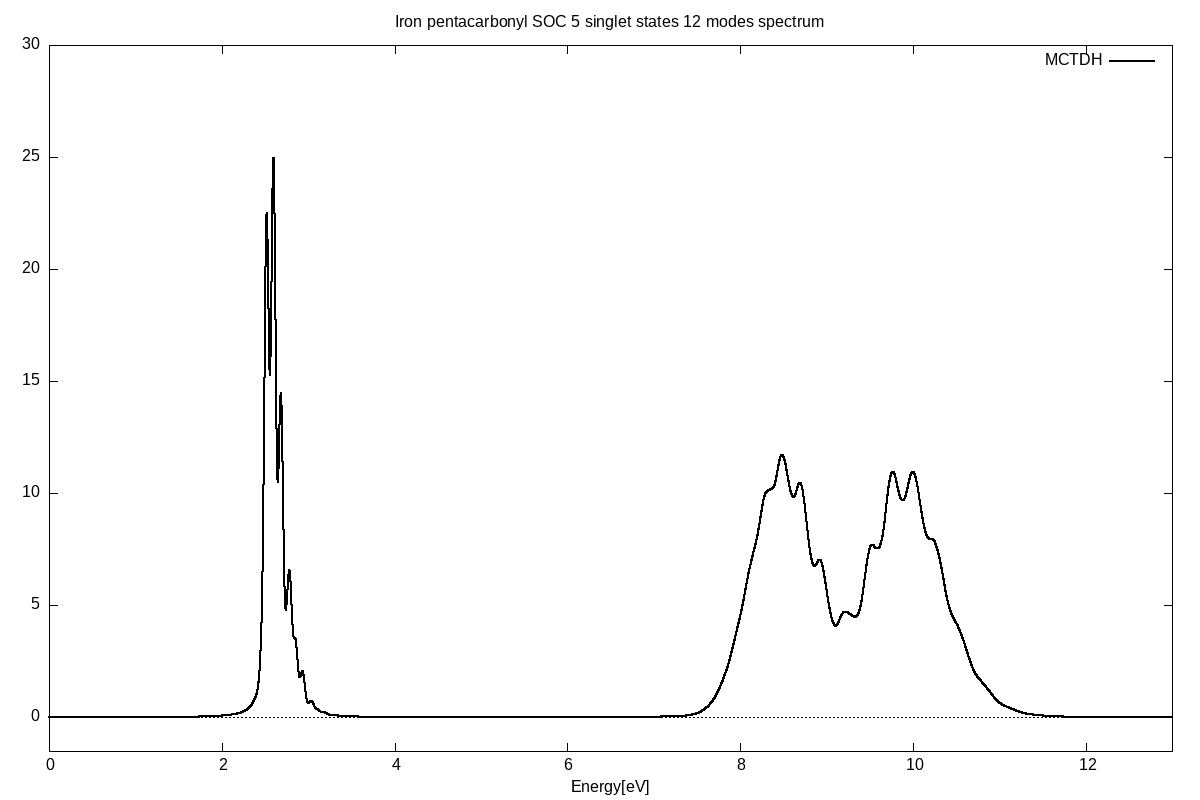
\includegraphics[width=1\columnwidth]{images/op_FeCO3Q_5st_PBF7_tf100.00_xyz_spectrum_5singlets.png}

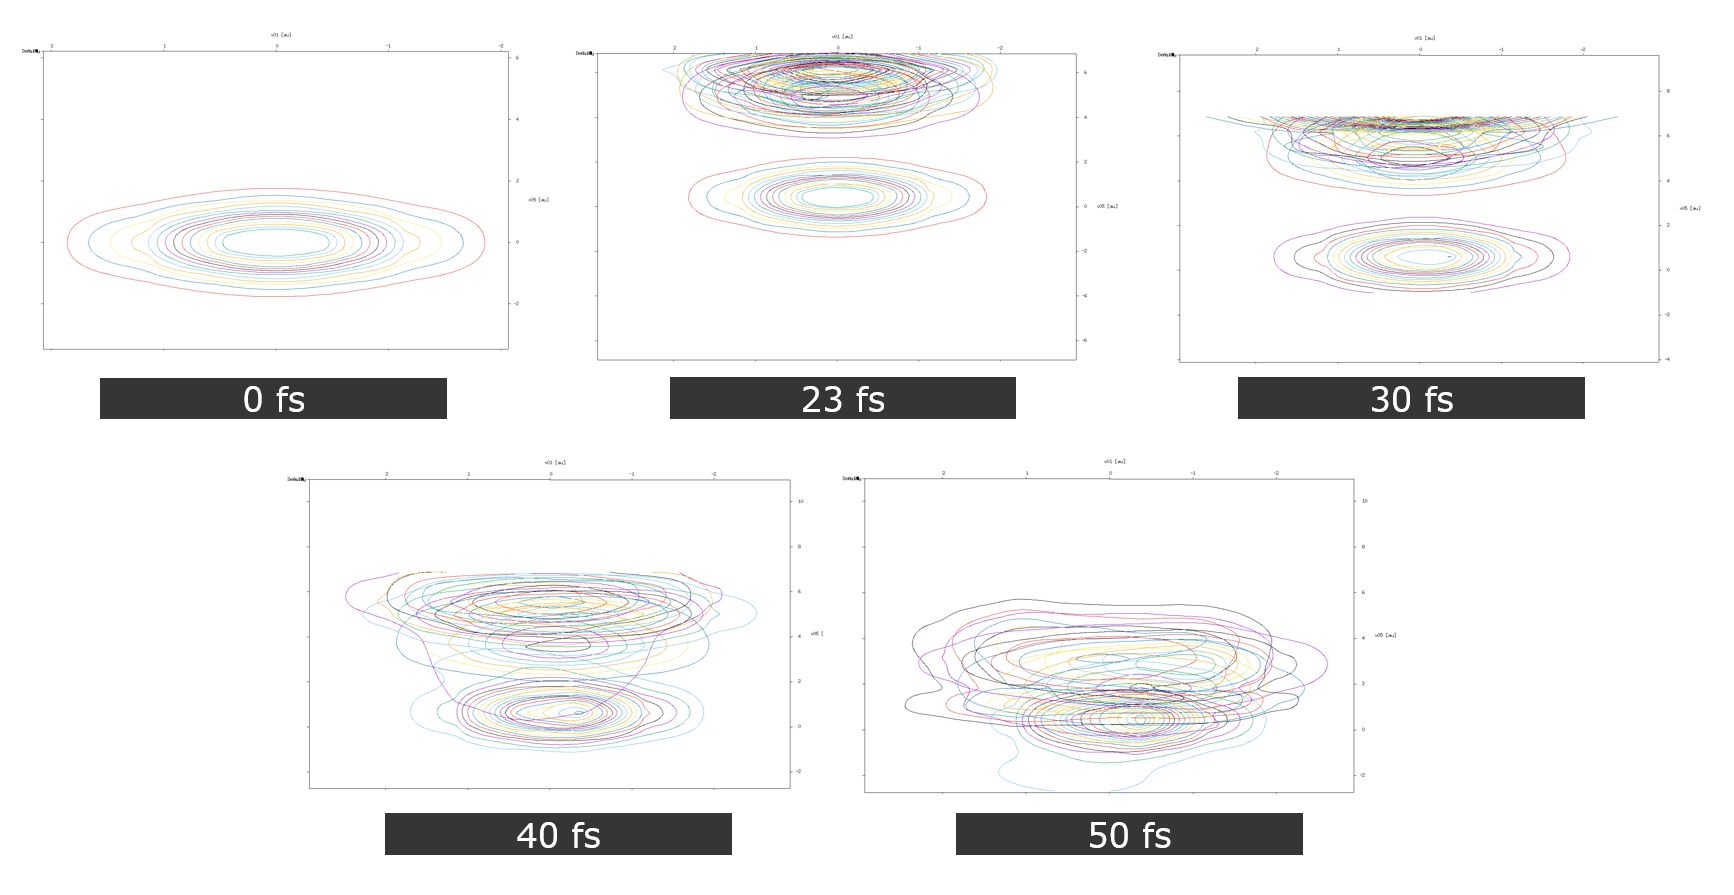
\includegraphics[width=1\columnwidth]{images/pes_progression.PNG}

\ce{D_{3h}} Character Table
\begin{table}[h]
\centering
\caption{Character Table for the $D_{3h}$ Point Group}
\begin{tabular}{c|cccccc}
\hline
$D_{3h}$ & $E$ & $2C_3$ & $3C'_2$ & $\sigma_h$ & $2S_3$ & $3\sigma_v$ \\
\hline
$A'_1$   & 1 &  1 &  1 &  1 &  1 &  1 \\
$A'_2$   & 1 &  1 & -1 &  1 &  1 & -1 \\
$A''_1$  & 1 &  1 &  1 & -1 & -1 & -1 \\
$A''_2$  & 1 &  1 & -1 & -1 & -1 &  1 \\
$E'$     & 2 & -1 &  0 &  2 & -1 &  0 \\
$E''$    & 2 & -1 &  0 & -2 &  1 &  0 \\
\hline
\end{tabular}
\label{tab:character_table_d3h}
\end{table}

\begin{lstlisting}
rdgpop86 1 0
 mode dof  dim   DVR     modelabel
   1    1    8   HO      v01
   1    2    8   HO      v02
   1    3   10   HO      v03
   1    4   10   HO      v04
   2    5   30   HO      v05
   2    6   20   HO      v06
   2    7   20   HO      v07
   3    8   30   HO      v08
   3    9   30   HO      v09
   3   10   30   HO      v10
   4   11   16   HO      v11
   4   12   12   HO      v12

 Maximal values (all times and states);  final time:     8.20 fs
   #  dof     grid(begin)    grid(end)      basis(begin)   basis(end)
   1  v01     0.003819209    0.004304504    1.000000000    0.069330648
   2  v02     0.002394854    0.002907799    1.000000000    0.094262965
   3  v03     0.006564292    0.011120993    1.000000000    0.054929234
   4  v04     0.008430379    0.007697208    1.000000000    0.060806006
   \textbf{5  v05     0.000016531    0.378852129    1.000000000    0.008608200}
   6  v06     0.000240223    0.018687338    1.000000000    0.000193951
   7  v07     0.000044060    0.046103045    1.000000000    0.000832838
   8  v08     0.030122789    0.021198401    1.000000000    0.007997538
   9  v09     0.053021628    0.015153312    1.000000000    0.010167416
  \textbf{10  v10     0.000000222    0.360995024    1.000000000    0.029714981}
  11  v11     0.001646049    0.000000013    1.000000000    0.000000208
  12  v12     0.000002498    0.001008901    1.000000000    0.000000019

******************************************************************************

rdcheck86 0 0

mode: No. of SPFs per state : modelabels
   1 :   6  10  10   8  12   1 :  v01 v02 v03 v04
   2 :   6   8   8   8   8   1 :  v05 v06 v07
   3 :   6  10  10  10  12   1 :  v08 v09 v10
   4 :   5   5   5   5   5   1 :  v11 v12

 tinit =      0.000 fs,    tout =      0.100 fs
--------------------------------------------------------------------------------
 Maximum over time of lowest nat.-weight;    time :      50.00 fs
 mode    s = 1      s = 2      s = 3      s = 4      s = 5      s = 6
   1   2.848E-03  7.210E-03  6.974E-03  9.912E-03  4.711E-03  0.000E+00
   2   2.567E-03  6.879E-03  7.224E-03  8.111E-03  8.778E-03  0.000E+00
   3   2.259E-03  9.978E-03  9.306E-03  6.689E-03  8.065E-03  0.000E+00
   4   8.478E-05  3.963E-06  6.035E-06  1.653E-05  4.295E-05  0.000E+00

\end{lstlisting}

No matter how much we tried to increase the primitive basis grid size, the end state is always highly populated, meaning that the potentials are unbound.


% \section{Tris(bipyridine)ruthenium(II) chloride, \ce{[Ru(bpy)3]Cl2}}
%     \subsection{https://en.wikipedia.org/wiki/Tris(bipyridine)ruthenium(II)_chloride}
    
% \section{https://pubs.acs.org/doi/10.1021/ic800091y}

% \section{Copper halides}

\newpage
\else \fi

\iffinalize \addcontentsline{toc}{chapter}{References / Bibliography} \chapter*{References / Bibliography} \newpage
%\renewcommand*{\bibfont}{\scriptsize}
\printbibliography
\else \fi

\iffinalize \addcontentsline{toc}{chapter}{Appendices} \chapter*{Appendices} \newpage
\begin{lstlisting}[
frame=single, numbers=left, firstnumber=1, backgroundcolor=\color{yellow!10},
label={lst:c1-overlap_matrix}, caption={\centering
    Toby Zeng's handcrafted \$REFDET group in \code{RhF3_SPK_gmcpt_C1_e_mult5_diis_15st_diab_refG.inp}
},
]
 $REFDET
  15
 1 1
      206   -1.000000
 2 4
      134   -0.500000
      167    0.500000
      186   -0.500000
       81    0.500000
 3 6
       59   -0.408248
       26   -0.408248
       98   -0.408248
       45    0.408248
      112    0.408248
      146   -0.408248
 4 4
        6   -0.500000
       11    0.500000
       31   -0.500000
       86    0.500000
 5 1
        1   -1.000000
 6 1
      207    1.000000
 7 4
       82    0.500000
      135   -0.500000
      168    0.500000
      196   -0.500000
 8 6
       99    0.408248
       46   -0.408248
      156    0.408248
       27    0.408248
      122   -0.408248
       69    0.408248
 9 4
        7   -0.500000
       16    0.500000
       91    0.500000
       36   -0.500000
 10 1
        2    1.000000
 11 1
      208    1.000000
 12 4
       83   -0.500000
      188   -0.500000
      136    0.500000
      197    0.500000
 13 6
      114    0.408248
      123   -0.408248
       61   -0.408248
      176    0.408248
       28    0.408248
       70    0.408248
 14 4
       13   -0.500000
      106    0.500000
       51   -0.500000
       17    0.500000
 15 1
        8    1.000000
 $END
\end{lstlisting}
\else \fi

\iffinalize \addcontentsline{toc}{chapter}{Glossary} \chapter*{Glossary} \newpage
\else \fi

\iffinalize \addcontentsline{toc}{chapter}{Index} \chapter*{Index} \newpage

Haruyuki Nakano. Hisao Nakamura.

SOC: https://pubs.aip.org/aip/jcp/article/146/14/144103/195065 Metal trifluorides: https://www.scie
Diabatic states: G. J. Atchity and K. Ruedenberg, Theor. Chem. Acc. 97, 47 (1997).https://doi.org/10.
https://pubs.aip.org/aip/jcp/article/115/22/10353/946057/The-direct-calculation-of-diabatic-
states-based-on
UV spectra: https://onlinelibrary.wiley.com/doi/10.1002/qua.10724
Linear vibronic models: https://pubs.acs.org/doi/10.1021/acs.jctc.1c00022 (Santoro)

We are using ORMAS+GMCPT! Student guide that really crystallized my knowledge of GMC-QDPT:
\url{ttps://ccl.scc.kyushu-u.ac.jp/~nakano/gmcpt.html}

% file:///Users/bjc/Downloads/configurational_uniformity_hisao.pdf - configurational uniformity paper

% J Comput Chem 23: 1166–1175, 2002 : GMC-QDPT paper
    
% \subsection{https://pubs.acs.org/doi/10.1021/jacs.2c01469} - this is the iron pentacarbonyl modern paper
% \subsection{https://pubs.acs.org/doi/10.1021/jp992474u}
% \subsection{https://pubs.aip.org/aip/jcp/article/75/6/2560/791508/The-Jahn-Teller-effect-in-the-photoelectron} \\

Iron pentacarbonyl, haruyuki nakano and mark s gordon https://pubs.rsc.org/en/content/articlepdf/1999/cp/a808518h


This is a very good diagram showing interdependencies: https://en.wikipedia.org/wiki/Complete\_active\_space\_perturbation\_theory

This is a good consideration for future work, running the calculations via GPU acceleration: 
https://www.nvidia.com/es-la/data-center/gpu-accelerated-applications/gamess/

MCTDH troubleshooting
% https://www.pci.uni-heidelberg.de/tc/usr/mctdh/doc.86/mctdh/trouble.html#redim 

% GAMESS input documentation: https://www.msg.chem.iastate.edu/gamess/GAMESS_Manual/docs-input.txt

\else \fi



\input{chapters/caveats}

\end{document}

